\begin{figure}
\centering
\begin{minipage}{.05\columnwidth}
\begin{flushleft}
    \raisebox{.2\height}{\rotatebox{90}{denoising}}
    \tikz \draw [-{Computer Modern Rightarrow[length=2mm, width=3mm]}, line width=.3mm] (0,2) -- (0,0); \\
\end{flushleft}
\end{minipage}~~
\begin{minipage}{.9\columnwidth}
\centering
    \vspace{.15cm}
    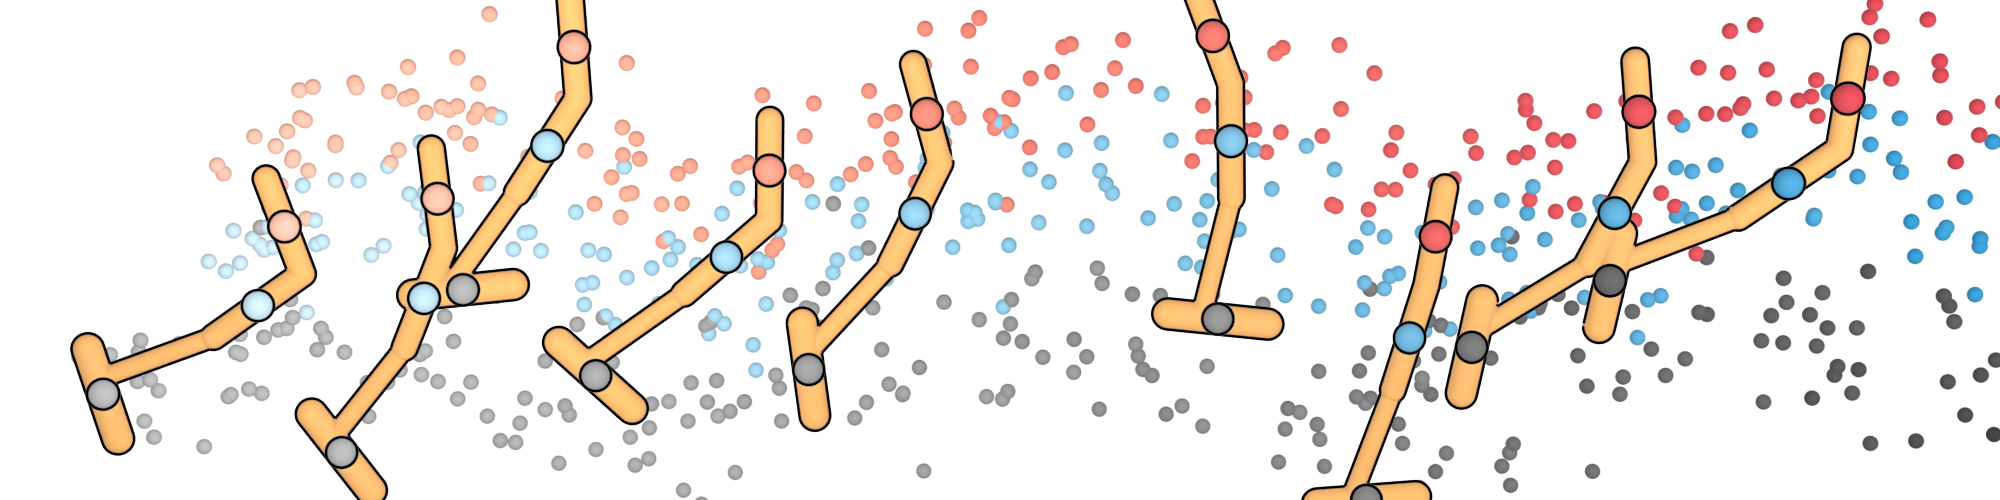
\includegraphics[width=\linewidth]{images/locomotion/merged-hopper-10.png} \\
    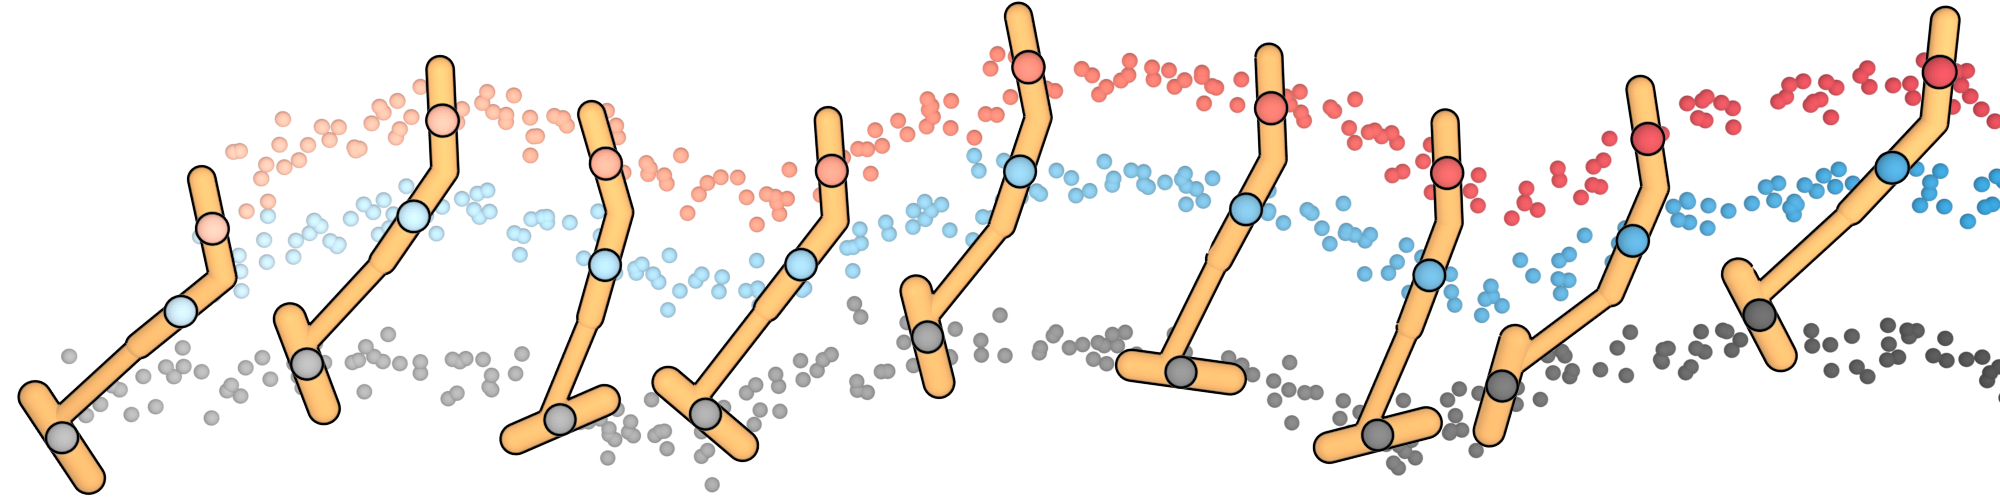
\includegraphics[width=\linewidth]{images/locomotion/merged-hopper-2.png} \\
    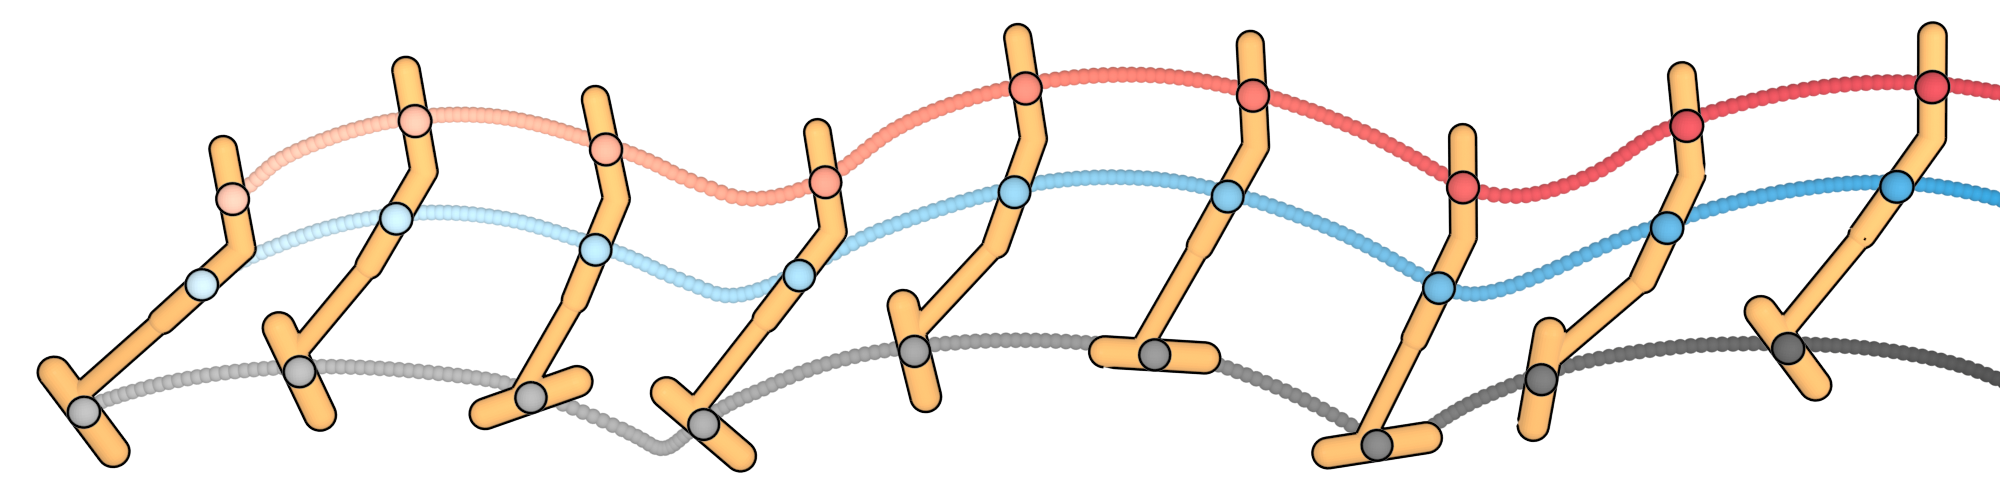
\includegraphics[width=\linewidth]{images/locomotion/merged-hopper-0.png} \\
\end{minipage} \\
\vspace{.3cm}
\hspace{1cm}
\raisebox{.3\height}{planning horizon}~~
\tikz \draw [-{Computer Modern Rightarrow[length=2mm, width=3mm]}, line width=.3mm] (0,0) -- (3,0); \\
\caption{
    \textbf{(Guided sampling)}
    \method generates all timesteps of a plan concurrently, instead of autoregressively, through the denoising process.
}
\vspace{-15pt}
\label{fig:locomotion}
\end{figure}